
% This LaTeX was auto-generated from an M-file by MATLAB.
% To make changes, update the M-file and republish this document.

\documentclass{article}
\usepackage{graphicx}
\usepackage{color}
\usepackage{listings}
\usepackage[framed]{mcode}
\usepackage{fullpage}
\usepackage{amsmath}
\usepackage[utf8x]{inputenc}
\usepackage{import}
\usepackage{setspace}
\usepackage{hyperref}
\definecolor{lightgray}{gray}{0.5}
\setlength{\parindent}{0pt}

\begin{document}

    
    
%\section*{}


\title{BE 521: Homework 2 Questions \\{\normalsize Modeling Neurons} \\{\normalsize Spring 2021}}
\author{46 points}
\date{Due: Tuesday, 2/9/2021 10:00 PM}
\maketitle
\textbf{Objective:} Computational modeling of neurons. \\
We gratefully acknowledge Dr. Vijay Balasubramanian (UPenn) for many of
the questions in this homework.\\


\begin{center}
\author{Shubhankar Patankar \\
  \normalsize Collaborators: Peter Galer \\}
\end{center}


\section{Basic Membrane and Equilibrium Potentials (6 pts)}
Before undertaking this section, you may find it useful to read pg.
153-161 of Dayan \& Abbott's \textit{Theoretical Neuroscience} (the
relevant section of which, Chapter 5, is posted with the homework).


\begin{enumerate}
 \item Recall that the potential difference $V_T$ when a mole of ions crosses a cell membrane is defined by the universal gas constant $R = 8.31\; {\rm J/mol\cdot K}$, the temperature $T$ (in Kelvin), and Faraday's constant $F = 96,480 {\rm\ C/mol}$ \[ V_T = \frac{RT}{F} \] Calculate $V_T$ at human physiologic temperature ($37\; ^{\circ} \rm C$). (1 pt)


\rule{\textwidth}{1pt}
\textit{Example Latex math commands that uses the align tag to make your equations
neater. You can also input math into sentences with \$ symbol like $\pi + 1$.}
\begin{align*}
E = MC^2 \tag{not aligned}\\
E = & MC^2 \tag{aligned at = by the \&}\\
1 = &\; \frac{2}{2}\tag{aligned at = by \&}
\end{align*}
\rule{\textwidth}{1pt}


 \item Use this value $V_T$ to calculate the Nernst equilibrium potentials
 (in mV) for the $\rm K^+$, $\rm Na^+$, and $\rm Cl^-$ ions, given the following
 cytoplasm and extracellular concentrations in the squid giant axon:
 $\rm K^+$ : (120, 4.5), $\rm Na^+$ : (15, 145), and $\rm Cl^-$ : (12, 120),
 where the first number is the cytoplasmic and the second the extracellular
 concentration (in mM). (2 pts)


 \item
  \begin{enumerate}
	\item Use the Goldmann equation,
	  \begin{equation}
		V_m = V_T\ln\left( \frac{\rm P_{K}\cdot[K^+]_{out} + P_{NA}\cdot[Na^+]_{out} + P_{Cl}\cdot[Cl^-]_{in}}{\rm P_{K}\cdot[K^+]_{in} + P_{NA}\cdot[Na^+]_{in} + P_{Cl}\cdot[Cl^-]_{out}} \right)
	  \end{equation}
	to calculate the resting membrane potential, $V_m$, assuming that the ratio of membrane permeabilities $\rm P_K:P_{Na}:P_{Cl}$ is $1.0:0.045:0.45$. Use the ion concentrations given above in Question 1.2. (2 pts)


	\item Calculate the membrane potential at the peak action potential, assuming a permeability ratio of $1.0:11:0.45$, again using the ion concentrations given in Question 1.2. (1 pt)
  \end{enumerate}


	\item The amplitudes of the multi-unit signals in HW0 and local field
	potentials (LFP) in HW1 had magnitudes on the order of 10 to 100
	microvolts. The voltage at the peak of the action potential (determined
	using the Goldman equation above) has a magnitude on the order of 10
	millivolts. Briefly explain why we see this difference in magnitude.
	Hint 1: Voltage is the difference in electric potential between two
	points. What are the two points for our voltage measurement in the
	multi-unit and LFP signals? What are the two points for the voltage
	measurement of the action potential? Hint 2: The resistance of the neuronal membrane is typically much higher than the resistance of the extracellular fluid. (2 pts)


\end{enumerate}
\section{Integrate and Fire Model (38 pts)}
You may find it useful to read pg.\ 162-166 of Dayan and Abbott for this section. The general differential equation for the integrate and fire model is
\[ \tau_m\frac{dV}{dt} = V_m - V(t) + R_m I_e(t) \]
where $\tau_m = 10\, \rm ms$ is the membrane time constant, describing how fast the current is leaking through the membrane, $V_m$ in this case is constant and represents the resting membrane potential (which you have already calculated in question 1.3.a), and $V(t)$ is the actual membrane potential as a function of time. $R_m = 10^7\, \Omega$ is the constant total membrane resistance, and $I_e(t)$ is the fluctuating incoming current. Here, we do not explicitly model the action potentials (that's Hodgkin-Huxley) but instead model the neuron's behavior leading up and after the action potential.


Use a $\Delta t = 10\, \rm \mu s$ ($\Delta t$ is the discrete analog of the continuous $dt$). Remember, one strategy for modeling differential equations like this is to start with an initial condition (here, $V(0)=V_m$), then calculate the function change (here, $\Delta V$, the discrete analog to $dV$) and then add it to the function (here, $V(t)$) to get the next value at $t+\Delta t$. Once/if the membrane potential reaches a certain threshold ($V_{th} = -50\, \rm mV$), you will say that an action potential has occurred and reset the potential back to its resting value.
\begin{enumerate}
 \item Model the membrane potential with a constant current injection (i.e., $I_e(t) = I_e = 2 {\rm nA}$). Plot your membrane potential as a function of time to show at least a handful of ``firings.'' (8 pts)

\begin{lstlisting}
tau_m = 10 * 10^-3; % s
V_m = -63.1 * 10^-3; % resting membrane potential (V)
V_th = -50 * 10^-3; % threshold voltage (V)
R_m = 10^7; % Ohm

sim_time = 0.1; % s
del_T = 10 * 10^-6; % time increment
time = 0:del_T:sim_time;

I_e = 2 * 10^-9; % A

V = zeros(1, length(time));
V(1) = V_m; % initial condition

for i = 1:length(time) - 1
    if V(i) > V_th
        V(i + 1) = V_m; % set to resting membrane potential
    else
        del_V = ((V_m - V(i) + R_m * I_e)/tau_m) * del_T;
        V(i + 1) = V(i) + del_V;
    end
end


figure;
plot(time * 10^3, V * 10^3, 'LineWidth', 2, 'Color', [0, 0, 0])
xlabel('Time (ms)', 'FontSize', 15);
ylabel('Membrane Potential (mV)', 'FontSize', 15);
\end{lstlisting}


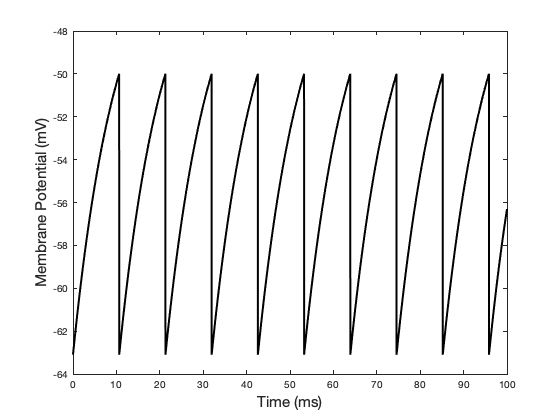
\includegraphics [width=5in]{spatank_hw2_01.png}

 \item Produce a plot of firing rate (in Hz) versus injection current, over the range of 1-4 nA. (4 pts)

\begin{lstlisting}
sim_time = 1; % s
del_T = 10 * 10^-6; % time increment
time = 0:del_T:sim_time;

I_e = (1:0.005:4) * 10^-9; % A
firing_rate = zeros(size(I_e));

V = zeros(1, length(time));
V(1) = V_m; % initial condition

for i = 1:length(I_e)
    I = I_e(i);
    action_potentials = 0;
    for j = 1:length(time) - 1
        if V(j) > V_th
            V(j + 1) = V_m; % set to resting membrane potential
            action_potentials = action_potentials + 1;
        else
            del_V = ((V_m - V(j) + R_m * I)/tau_m) * del_T;
            V(j + 1) = V(j) + del_V;
        end
    end
    firing_rate(i) = action_potentials;
end

figure;
plot(I_e * 10^9, firing_rate, 'LineWidth', 2, 'Color', [0, 0, 0])
xlabel('Injected Current (nA)', 'FontSize', 15);
ylabel('Firing Rate (Hz)', 'FontSize', 15);
\end{lstlisting}


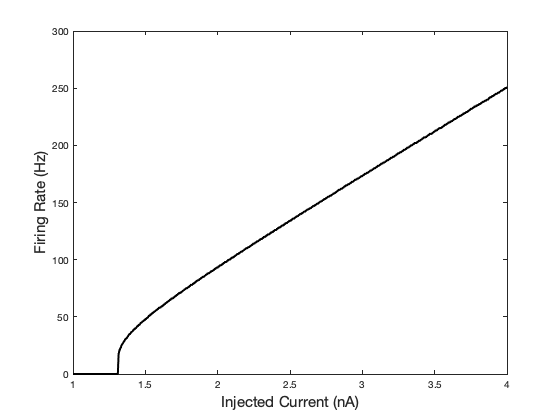
\includegraphics [width=5in]{spatank_hw2_02.png}

 \item \texttt{I521\_A0002\_D001} contains a dynamic current injection in nA. Plot the membrane potential of your neuron in response to this variable injection current. Use Matlab's \texttt{subplot} function to place the plot of the membrane potential above the injection current so that they both have the same time axis. (Hint: the sampling frequency of the current injection data is different from the sampling frequency ($\frac{1}{\Delta t}$) that we used above.) (4 pts)

\begin{lstlisting}
cd('/Users/sppatankar/Developer/BE-521')
addpath(genpath('ieeg-matlab-1.14.49'))
addpath(genpath('Homework_2'))

session = IEEGSession('I521_A0002_D001', 'spatank', 'spa_ieeglogin.bin');
sampling_rate = session.data.sampleRate; % Hz
end_time = session.data.rawChannels(1).get_tsdetails.getEndTime/1e6; % s

I_e_dyn = session.data.getvalues(1:ceil(end_time * sampling_rate), 1) * 10^-9; % A

del_T = 1/sampling_rate;
time = 0:del_T:end_time;

V = zeros(1, length(time));
V(1) = V_m; % initial condition

for i = 1:length(time) - 1
    if V(i) > V_th
        V(i + 1) = V_m; % set to resting membrane potential
    else
        del_V = ((V_m - V(i) + R_m * I_e_dyn(i))/tau_m)*del_T;
        V(i + 1) = V(i) + del_V;
    end
end

figure;
subplot(2, 1, 1);
plot(time * 10^3, V * 10^3, 'LineWidth', 2, 'Color', [0, 0, 0])
xlabel('Time (ms)', 'FontSize', 15);
ylabel('Membrane Potential (mV)', 'FontSize', 15);

subplot(2, 1, 2);
plot(time(1:end-1) * 10^3, I_e_dyn * 10^9, 'LineWidth', 2, 'Color', [0, 0, 0])
xlabel('Time (ms)', 'FontSize', 15);
ylabel('Injected Current (nA)', 'FontSize', 15);


% Store these variables for easy access in Q2P5
sampling_rate_q2p3 = sampling_rate;
time_q2p3 = time;
V_q2p3 = V;
\end{lstlisting}

\color{lightgray} \begin{lstlisting}IEEGSETUP: Adding 'ieeg-matlab.jar' to dynamic classpath
IEEGSETUP: Found log4j on Java classpath.
URL: https://www.ieeg.org/services
Client user: spatank
Client password: ****
\end{lstlisting} \color{black}


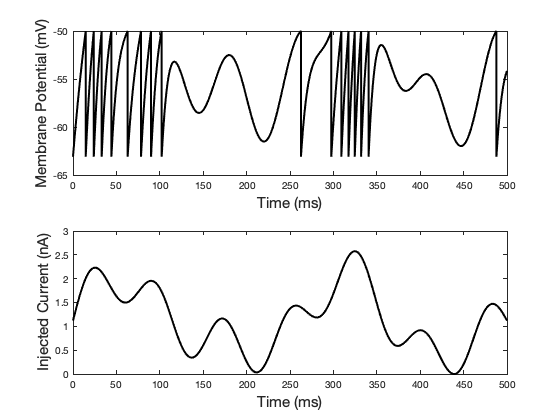
\includegraphics [width=5in]{spatank_hw2_03.png}

 \item Real neurons have a refractory period after an action potential that prevents them from firing again right away. We can include this behavior in the model by adding a spike-rate adaptation conductance term, $g_{sra}(t)$ (modeled as a potassium conductance), to the model
 \[ \tau_m\frac{dV}{dt} = V_m - V(t) - r_m g_{sra}(t)(V(t)-V_K)+ R_m I_e(t) \]
 where \[ \tau_{sra}\frac{dg_{sra}(t)}{dt} = -g_{sra}(t), \]
 Every time an action potential occurs, we increase $g_{sra}$ by a certain constant amount, $g_{sra} = g_{sra} + \Delta g_{sra}$. Use $r_m \Delta g_{sra} = 0.06$. Use a conductance time constant of $\tau_{sra} = 100\, \rm ms$, a potassium equilibrium potential of $V_K = -70\, \rm mV$, and $g_{sra}(0) = 0$. (Hint: How can you use the $r_m \Delta g_{sra}$ value to update voltage and conductance separately in your simulation?)


 \begin{enumerate}
  \item Implement this addition to the model (using the same other parameters as in question 2.1) and plot the membrane potential over 200 ms. (8 pts)

\begin{lstlisting}
sim_time = 0.2; % s
del_T = 10 * 10^-6; % time increment
time = 0:del_T:sim_time;

I_e = 2 * 10^-9; % A

V = zeros(1, length(time));
V(1) = V_m; % initial condition

tau_sra = 100 * 10^-3; % s
V_K = -70 * 10^-3; % (V)

r_g_sra = zeros(1, length(time));
r_g_sra(1) = 0;

for i = 1:length(time) - 1
    if V(i) > V_th
        V(i + 1) = V_m; % set to resting membrane potential
        r_g_sra(i + 1) = r_g_sra(i) + 0.06;
    else
        del_V = (V_m - V(i) - (r_g_sra(i) * (V(i) - V_K)) + (R_m * I_e)) * (del_T / tau_m);
        V(i + 1) = V(i) + del_V;
        del_r_g_sra = -r_g_sra(i) * (del_T / tau_sra);
        r_g_sra(i + 1) = r_g_sra(i) + del_r_g_sra;
    end
end


figure;
plot(time * 10^3, V * 10^3, 'LineWidth', 2, 'Color', [0, 0, 0])
xlabel('Time (ms)', 'FontSize', 15);
ylabel('Membrane Potential (mV)', 'FontSize', 15);
\end{lstlisting}


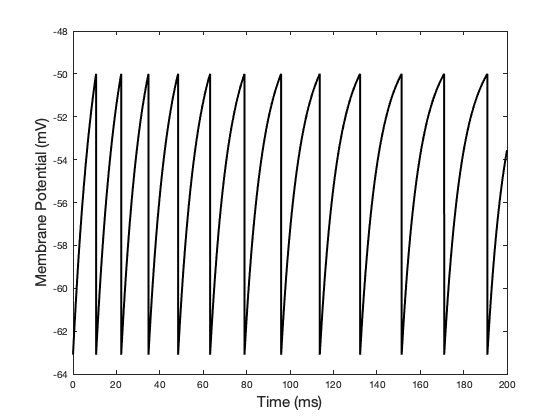
\includegraphics [width=5in]{spatank_hw2_04.png}

  \item Plot the inter-spike interval (the time between the spikes) of all the spikes that occur in 500 ms. (2 pts)

\begin{lstlisting}
sim_time = 0.5; % s
del_T = 10 * 10^-6; % time increment
time = 0:del_T:sim_time;

I_e = 2 * 10^-9; % A

V = zeros(1, length(time));
V(1) = V_m; % initial condition

r_g_sra = zeros(1, length(time));
r_g_sra(1) = 0;

spike_times = [];

for i = 1:length(time) - 1
    if V(i) > V_th
        V(i + 1) = V_m; % set to resting membrane potential
        r_g_sra(i + 1) = r_g_sra(i) + 0.06;
        spike_times = [spike_times, time(i)];
    else
        del_V = (V_m - V(i) - (r_g_sra(i) * (V(i) - V_K)) + (R_m * I_e)) * (del_T / tau_m);
        V(i + 1) = V(i) + del_V;
        del_r_g_sra = -r_g_sra(i) * (del_T / tau_sra);
        r_g_sra(i + 1) = r_g_sra(i) + del_r_g_sra;
    end
end

inter_spike_interval = diff(spike_times) * 10^3;

figure;
plot(1:length(inter_spike_interval), inter_spike_interval, 'LineWidth', 2, 'Color', [0, 0, 0])
xlabel('Spike Pair', 'FontSize', 15);
ylabel('Inter-spike Interval (ms)', 'FontSize', 15);

figure;
plot(time * 10^3, r_g_sra, 'LineWidth', 2, 'Color', [0, 0, 0])
xlabel('Time (ms)', 'FontSize', 15);
ylabel('rg_{sra}', 'FontSize', 15);
\end{lstlisting}


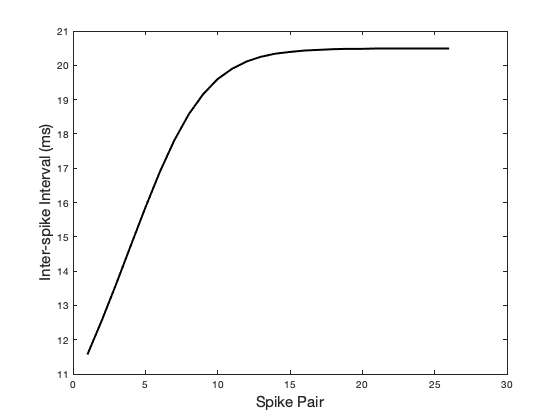
\includegraphics [width=5in]{spatank_hw2_05.png}


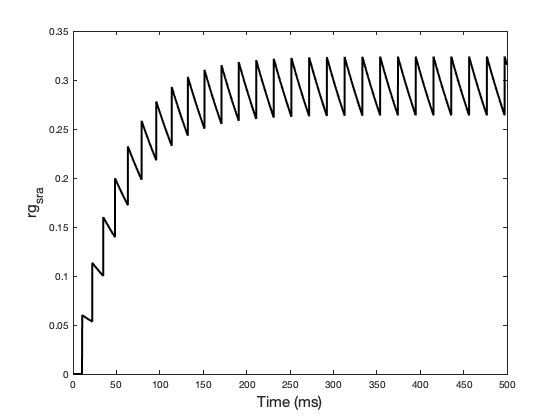
\includegraphics [width=5in]{spatank_hw2_06.png}

  \item Explain how the spike-rate adaptation term we introduced above might be contributing to the behavior you observe in 2.4.b. (2 pts)


 \end{enumerate}
 \item Pursue an extension of this basic integrate and fire model. A few ideas are: implement the Integrate-and-Fire-or-Burst Model of Smith et al.\ 2000 (included); implement the Hodgkin-Huxley model (see Dayan and Abbot, pg.\ 173); provide some sort of interesting model of a population of neurons; or perhaps model what an electrode sampling at 200 Hz would record from the signal you produce in question 2.3. Feel free to be creative.
 We reserve the right to give extra credit to particularly interesting extensions and will in general be more generous with points for more difficult extensions (like the first two ideas), though it is possible to get full credit for any well-done extension.
  \begin{enumerate}
	\item Briefly describe what your extension is and how you will execute it in code. (6 pts)

\begin{lstlisting}
clearvars -except sampling_rate_q2p3 time_q2p3 V_q2p3

sampling_rate_new = 200; % Hz
sample_rate_dec_factor = sampling_rate_q2p3/sampling_rate_new;

time_new = downsample(time_q2p3, sample_rate_dec_factor);
V_new = downsample(V_q2p3, sample_rate_dec_factor);

figure;
hold on
% subplot(2, 1, 1);
plot(time_q2p3 * 10^3, V_q2p3 * 10^3, 'LineWidth', 2, 'Color', [0.7, 0.7, 0.7])
xlabel('Time (ms)', 'FontSize', 15);
ylabel('Membrane Potential (mV)', 'FontSize', 15);


% subplot(2, 2, 3);
plot(time_new * 10^3, V_new * 10^3, 'LineWidth', 2, 'Color', [0, 0, 0])
xlabel('Time (ms)', 'FontSize', 15);
ylabel('Membrane Potential (mV)', 'FontSize', 15);
legend('Original', 'Downsampled');
hold off
\end{lstlisting}


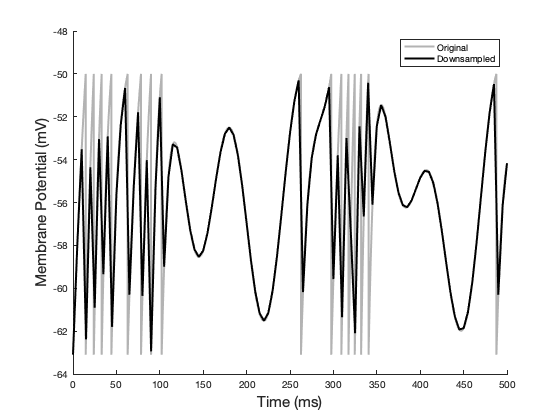
\includegraphics [width=5in]{spatank_hw2_07.png}

	\item Provide an interesting figure along with an explanation illustrating the extension. (4 pts)


  \end{enumerate}
\end{enumerate}




\end{document}
    
